\section{绪\hspace{1em}论}

本章我们首先介绍了当前图神经网络(Graph Neural Network, GNN)的技术发展趋势,然后分析了GNN的现有实现所存在的问题,
介绍了国内外在GNN加速领域的相关研究工作,并对本文的主要研究内容及工作意义作了具体说明。
\subsection{课题背景、目的与意义}
% 绪论主要介绍本文的选题背景:说明本设计课题的来源、目的、意义、应解决的主要问题及应达到的技术要求;
% 简述本课题在国内外发展概况及存在的问题,本设计的指导思想等。(原则上,这一章内容主要来自于开题报告)

% 论文中不允许出现“我”、“我们”、“本文”之类的词,可以用“本课题”或者“本研究”,甚至可以直接用无主句。
\subsubsection{研究背景与趋势}
% \begin{enumerate}
%     \item 参考文献必须全部在论文正文中按顺序引用
%     \item 不得在标题处进行引用,引用出现在标点之前。
%     \item 可以在引用处右上角加标注进行引用,也可以直接在正文中用“文献[3]指出……”这样的话语进行引用
%     \item 参考文献在后 面的【参考文献】中排列顺序按照在论文中第一次引用的先后顺序排列
%     \item 多篇参考文献群引不超过3篇,可使用如下风格:[1,2,3]、[1][2][3]
% \end{enumerate}
图结构数据(Graph-structured Data)在现实世界中无处不在,从社交网络、蛋白质相互作用网络、知识图谱到交通流网络和金融交易网络。如何有效地从这些图结构数据中学习和提取有价值的知识,已成为机器学习和数据挖掘领域的核心挑战之一。在此背景下,图神经网络(Graph Neural Network, GNN)应运而生,并迅速成为处理图数据的强大范式。GNN通过迭代地聚合邻居节点信息来更新节点表示,能够有效地捕捉图的拓扑结构和节点特征,在节点分类、链接预测、图分类等多种任务中取得了突破性进展,并在推荐系统、药物发现、自然语言处理、计算机视觉等众多领域展现出巨大的应用潜力。

与传统图分析方法(如随机游走~\cite{grover2016node2vec, deepWalk}和图拉普拉斯方法~\cite{luo2011cauchy, luo2009non})相比,图神经网络通过独特的“聚合-更新”双阶段交替执行机制脱颖而出:在“聚合”阶段执行图操作(如分散-收集,scatter-gather),在“更新”阶段执行神经网络操作(矩阵乘法),从而显著提升准确率并增强泛化能力。然而,GNN的独特机制也为GNN框架的设计与实现带来了许多问题和挑战。现有支持GNN训练与推理的研究可分为两类:第一类基于图处理系统扩展神经网络功能,第二类则从深度学习框架扩展图操作支持。但这些方案仍存在诸多局限性,如对图数据的支持不足、对GNN模型的支持不全面,不能有效利用GNN的运行时信息进行优化,导致在处理大规模图数据时性能瓶颈明显,在面对不断增大的图规模和多样化的节点嵌入维度时表现欠佳。

图形处理器(Graphics Processing Units, GPU)凭借其大规模并行计算能力和高内存带宽,已从最初的图形渲染专用硬件发展成为通用并行计算(General-Purpose computing on GPUs, GPGPU)的主流平台,尤其在深度学习领域取得了巨大成功。GPU的架构特点使其非常适合处理计算密集型和数据并行的任务。本课题选取GPU作为研究对象,旨在通过对GPU架构的深入分析,探索其在图神经网络加速中的应用潜力。本课题将重点关注GPU的并行计算能力、内存访问模式和负载划分等方面,为GNN的高效实现提供新的思路和方法。

\subsubsection{面临的问题和挑战}
尽管GPU为GNN计算提供了强大的硬件基础,但要充分利用硬件的计算能力,将GNN高效地映射到GPU架构上,仍然面临一系列严峻的挑战:

\textbf{GNN的计算负载混合且高度不规则}:GNN包含聚合和更新两阶段。其中,聚合阶段是性能的关键瓶颈,其计算模式具有高度的不规则性:
\begin{itemize}
    \item \textit{内存访问不规则}: 访问邻居节点的特征数据通常是非连续、随机的,这与GPU内存系统为优化连续、规整访问(Coalesced Access)而设计的机制相冲突,导致内存带宽利用率低下,缓存效率差。
    \item \textit{计算量不规则}: 图中节点度数的幂律分布~\cite{graph-power-law}导致不同节点的邻居聚合计算量差异巨大。将节点或边直接映射到GPU线程或线程块进行处理,会引发严重的负载不均衡问题。部分处理高密度节点的线程或块成为性能瓶颈,而大量处理低密度节点的线程或块则提前完成并空闲,极大地降低了GPU的整体利用率~\cite{han2014experimental}。
\end{itemize}

\textbf{GPU并行执行模型的挑战}:GPU的SIMT执行模型要求一个Warp(通常32个线程)中的所有线程执行相同的指令。然而,在GNN计算中,由于负载不均衡或需要根据节点或边属性执行不同的处理逻辑(例如,处理不同类型的边或根据节点度选择不同聚合策略),容易导致同一Warp内的线程执行不同的代码分支,产生Warp发散。这会使部分线程被暂时屏蔽,降低了计算资源的有效利用率。

在GNN的聚合阶段,多个线程可能需要更新同一个目标节点的累积特征值,这通常需要使用原子操作(Atomic Operations)来保证数据一致性。在具有数千个并发线程的GPU上,高并发的原子操作会产生显著的竞争和串行化,成为性能瓶颈,尤其是在高节点度的情况下。

\textbf{现有GNN系统与框架的局限性}:当前许多GNN框架~\cite{pyG,wang2019dgl}依赖通用的稀疏计算库(如torch-scatter~\cite{torch-scatter})或标准的稀疏矩阵运算库(如cuSPARSE中的SpMM~\cite{cusparse})来实现图聚合操作。这些通用计算库往往没有针对GNN特有的数据访问模式和计算流程进行深度优化,导致性能不理想。
%例如,简单scatter add操作可能涉及大量的原子操作开销。

最优的GPU执行策略(如线程映射方式、共享内存使用策略、数据布局等)强烈依赖于具体的GNN模型、嵌入维度大小以及输入图的拓扑特性(如度分布、社区结构等)。GNN系统与框架如何感知输入特性并自动调整优化策略,在不同应用场景下应用不同的优化,充分利用GPU的计算资源,以达到最佳效果,是学界和工业界亟待解决的难题。

\subsubsection{课题目的与意义}
本课题的主要研究目的在于设计并实现一个面向GPU平台的高效、自适应的GNN计算加速运行时系统:~\Mname{}。~\Mname{}利用PyTorch作为前端,以便于用户使用和集成。在底层,~\Mname{}使用C++/CUDA构建,通过Python绑定到PyTorch,提供高效的GNN计算内核。数据由 Pytorch 编写的数据加载器加载,并以张量形式传递给 ~\Mname{},以便在 GPU 上进行计 算。一旦 ~\Mname{}d-visor 在 GPU 上完成计算,它就会将数据张量(tensor)传回原始 Pytorch 框架进行进一步处理。如图~\ref{fig: Overview}所示, ~\Mname{} 由几个关键组件组成,以促进 GNN 优化和在 GPU 上的执行。首先,~\Mname{} 引入了一个输入加载器和提取器(input Loader \& Extractor),以利用输入级信息来指导我们的系统级优化。其次,~\Mname{} 引入了一个由分析模型组成的 Decider,用于自动选择运行时参数,以减少设计优化过程中的人工操作,并加入了一个轻量级节点重编号例程,以提高图结构的局部性。第三,~\Mname{} 集成了内核与运行时创建(Kernel\&Runtime Crafter),用于定制参数化 GNN 内核和 CUDA 运行时,其中包括高效的二维负载管理(同时考虑邻节点数量和节点嵌入维度)和一套 GNN 专用内存优化。

 %  内核与运行时创建(Kernel\&Runtime Crafter)说的嫩牛逼其实就是pytorch提供的AT_DISPATCH_FLOATING_TYPES宏用于在运行时根据float和double类型展开template
 
\begin{figure}[htbp] 
    \centering
    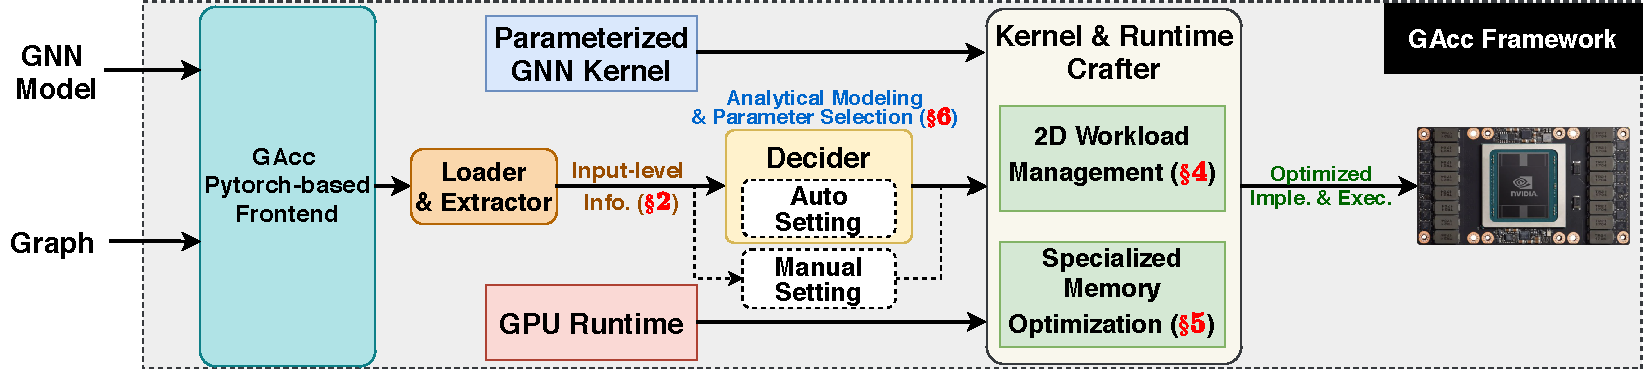
\includegraphics[width=\linewidth]{images/Overall-Arch-1.pdf}
    \caption{~\Mname{}的整体架构}
    \label{fig: Overview}
\end{figure}

本研究的顺利完成具有重要的理论价值和显著的实际应用意义。最直接地,它有望显著提升GNN在GPU上的计算效率,大幅缩短训练和推理时间。此外,虽然本课题侧重于GNN的加速,但是提出的自适应优化机制和负载均衡策略也可以推广到其他图计算任务和深度学习模型中,具有广泛的适用性和参考价值。通过深入研究GNN在GPU上的实现,本课题将为未来更高效的图计算框架和算法设计提供有益的启示。

\subsection{国内外研究现状}
% 通过大量文献阅读,对所研究内容进行综述,较为详细的说明研究内容的国内外现状,
% 建议按照时间轴分阶段说明或者按照原理/机制分类别说明,不论哪种方式,
% 都要对每个阶段/每个类别的工作原理、机制、试图解决的问题、解决了的问题和存在的不足进行阐述和分析,
% 该部分篇幅在3-4页为宜

% 一次引用建议不要超过三篇文献,文献引用按照:递增顺序、全部引用的原则进行引用
\subsubsection{通过算法加速GNN}
GNN训练加速的核心思想在于减少计算图的规模。同时,理想的加速训练方法应当能够在模型性能上达到与未经加速的常规训练方法相近的结果。在本节中,我们讨论两类主流的GNN训练加速技术:图修改(graph modification)和采样(sampling)。这两种方法都旨在通过缩减计算图来加速训练过程。它们的主要区别在于是否显式地生成一个修改后的图作为中间输出。
%对于图修改方法,其过程通常可以分为两个阶段。第一阶段处理原始图 ,输出一个规模更小、能够被快速处理和训练的新图 。第二阶段则以这个修改后的图 作为输入,进行常规的GNN训练。对于采样方法,它在每次训练迭代中动态地选择一部分节点或边的子集,用以构建规模更小的计算图。从广义上讲,采样也改变了原图的结构,但这种修改是动态且隐式(dynamically and implicitly)完成的,不会产生一个固定的中间图 。由于每次迭代构建的计算图可能不同,理论上通过足够多的迭代,原始图中的所有节点和边都有机会被采样覆盖。相比之下,图修改方法生成的 可能不会包含原始图中的所有节点和边,但有时也可能会引入新的节点或边结构。

\textbf{图修改}通过两个步骤加速GNN训练。第一阶段处理原始图 ,输出一个规模更小、能够被快速处理和训练的新图 。第二阶段则以这个修改后的图作为输入,进行常规的GNN训练。接下来本文将介绍三类图结构修改方法:图粗化(graph coarsening)、图稀疏化(graph sparsification)和图压缩(graph condensation)。这些方法通过不同策略生成各异的图,但其核心目标均为构建规模更小的训练图以提升 GNN 训练效率。图~\ref{figure:modification}直观展示了这些图修改方法的实现原理。
\begin{figure}[htbp]
    \begin{center}
    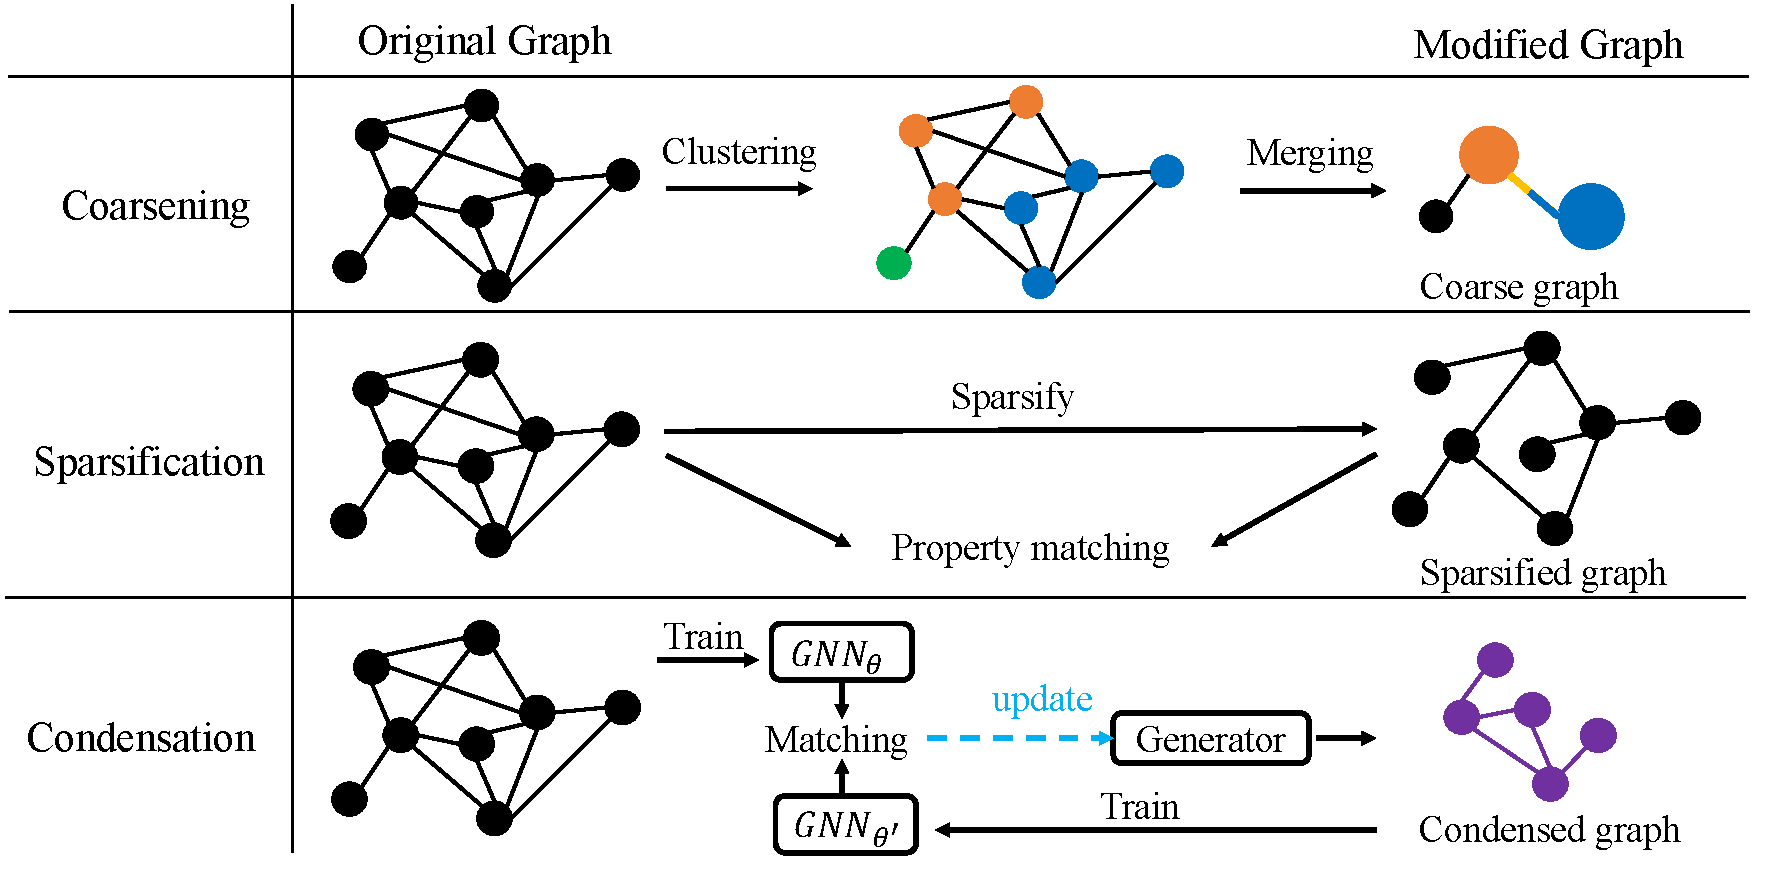
\includegraphics[width=\textwidth]{images/modification.pdf}
    \end{center}
    \caption{\textbf{图修改}方法图示:\textit{图粗化} (Graph Coarsening) 方法执行图聚类并将节点簇合并成超节点。\textit{图稀疏化} (Graph Sparsification) 方法移除不太重要的边。\textit{图压缩} (Graph Condensation) 方法使用一个随机初始化的生成模型来生成一个新的压缩图。对于修改后的图(最右列),黑色节点/边来自原始图,彩色节点/边是新创建的。}
    \label{figure:modification}
    \end{figure}
\begin{itemize}
    \item \textit{图粗化},是一种减小图大小同时保留其整体结构的技术。通过将相同局部结构中的节点合并为“超级节点”,并将连接超级节点的边合并为“超级边”,可以得到粗图。图粗化的核心步骤是图聚类,通常与图谱相关。一些算法如受限谱近似~\cite{loukas_coarsening2018}和逆拉普拉斯~\cite{bravo2019unifying},被用于保留一些图属性。
    \item \textit{图稀疏化},通过删除冗余边来减少计算图,加速GNN训练。现有方法通常保留原始图的关键属性,如切割总权重、光谱特性和分层结构。稀疏化算法可作为预处理步骤,降低全批次时间复杂度。现有图疏解方法保留的属性示例包括切分的总权重~\cite{benczur1996approximating}、谱属性~\cite{spielman2011graph,spielman2014nearly}和层次结构~\cite{serrano2009extracting}。一些相关工作执行基于GNN的图稀疏化以提高GNN精度或鲁棒性,但这些方法通常需要解决额外的优化问题,可能减慢训练速度。
    \item \textit{图压缩},通过匹配两个GNN的训练梯度来生成一个压缩图,从而减少GNN的计算量和内存占用。GCond~\cite{jin2021graph}是一种具有代表性的用于生成压缩图的方法,可以在保留原始图训练动态的同时显著减小图的大小。通过在原始图和压缩图上训练两个具有相同架构的GNN,GCond可以生成压缩图,同时保持原始GNN的性能。实验表明,GCond可以在多个图基准上实现小于$1\%$的压缩比,同时保持原始GNN超过$95\%$的准确度。因此,GCond非常适合神经架构搜索等任务。然而,为了加速单个GNN的训练,GCond应该与其他加速方法或更好的压缩策略相结合。
\end{itemize}

\textbf{图采样}每次训练迭代中动态地选择一部分节点或边的子集,用以构建规模更小的计算图。需要注意的是,采样与图形修改不同,采样是动态且隐式的,没有中间修改的图形输出。采样方法分为节点方式、逐层和子图方式三类,图\ref{figure:sampling}这三种采样算法的工作流程。
\begin{figure}[htbp]
    \begin{center}
    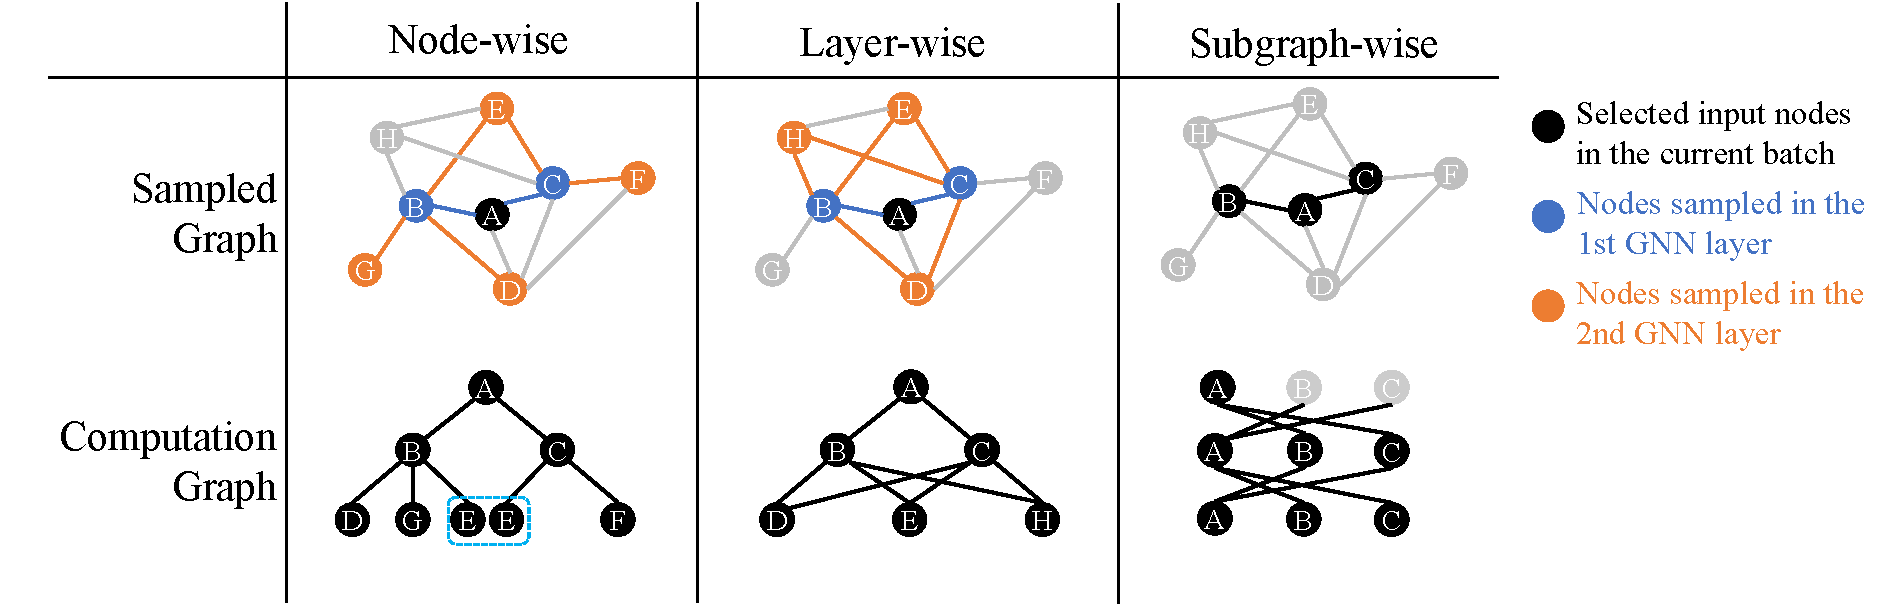
\includegraphics[width=\textwidth]{images/sampling.pdf}
    \end{center}
    \caption{\textbf{图采样}方法的示意图。\textit{节点级采样}(Node-wise Sampling)方法为每个计算层的每个节点单独采样,可能导致节点冗余(如节点E被重复采样两次)和边缺失(如节点C与D之间的边缺失);\textit{层级采样}(Layer-wise Sampling)方法基于前一层的节点进行逐层采样;\textit{子图级采样}(Subgraph-wise Sampling)方法通过采样节点列表及其诱导子图,在采样得到的子图内部沿所有边进行消息传递。}
    \label{figure:sampling}
\end{figure}
\begin{itemize}
    \item \textit{节点方式},通过选择一部分节点来构建一个子图。该方法的关键在于如何选择节点。现有方法通常基于节点的特征或连接性进行选择。GNN 算法加速中的节点采样方法,旨在通过减少聚合操作中涉及的邻居节点数量来降低计算复杂度。GraphSAGE~\cite{sage} 是该领域的开创性工作。它在 GNN 的每一层为每个目标节点从其全部邻居中均匀地采样固定数量的节点,构成采样后的邻居集。GraphSAGE 使用这个较小的邻居集来进行聚合计算,而不是使用全部邻居,从而显著减少了计算开销,加速了 GNN 的处理过程。重要的是,通过调整采样节点贡献的权重,这种采样聚合是对使用全邻居聚合结果的无偏估计,保证了采样方法的理论正确性。
    \item \textit{逐层方式},通过逐层地选择节点和边来构建子图。该方法通常使用随机游走或邻居采样等技术来选择节点和边。FastGCN~\cite{chen2018fastgcn}首次提出了分层重要性采样方案,以解决分节点采样的可扩展性问题。AS-GCN~\cite{huang2018adaptive}提出了一种自适应分层采样方法,以加速大规模图上 GCN 的训练。该方法以顶层为条件对下层进行采样,采样邻域由不同的父节点共享,避免了过度扩展。
    \item \textit{子图方式},通过选择一部分子图来构建一个新的计算图。由于子图通常较小且只表示局部信息,训练时需要添加随机性以提高准确性。这些方法与图修改方法类似,但并非真正修改图,而是动态采样。GraphSAINT~\cite{zeng2019graphsaint}是一种广泛使用的子图采样方法,它首先对节点进行采样,然后构建由采样节点诱导的子图。GraphSAINT 提出了四种不同的节点采样算法。在所提出的四种算法中,对随机节点集进行随机漫步,并在漫步中选择节点的随机漫步采样器的经验表现更好,因此得到了更广泛的应用。同直接在节点级别采样的GraphSAGE相比,构建子图的过程引入了额外的开销。ClusterGCN~\cite{chiang2019cluster} 采用图聚类算法(如 METIS~\cite{metis})将整个输入图划分为多个簇。每个簇内的节点构成连接紧密的子图,而簇间的边则被最小化。随后,ClusterGCN 在每个子图簇上进行全批量 (full-batch) GNN 训练。这种方法的一个局限性是聚类结果是固定的,导致训练过程中会丢失簇间的边。
\end{itemize}
\subsubsection{通过现有硬件系统加速GNN}
除了高效的GNN训练/推理算法,优化底层系统对于提高GNN的端到端吞吐量至关重要。现有工作从三个方面加速GNN系统:GPU内核加速、用户定义函数(UDF)优化和可扩展训练系统。由于GNN计算遵循消息传递范式,需要高效的稀疏操作,人们提出了各种高效的GNN内核和UDF优化技术。如何设计一个高效的可扩展 GNN 训练系统,仍然是机器学习系统界的一个开放研究问题。
\begin{itemize}
    \item \textit{GPU内核加速}。GPU作为高性能硬件加速器,可显著提升深度学习训练与推理中的计算效率。经过针对性优化的GPU内核(GPU kernels)GPU已广泛应用于深度学习加速领域,但由于图数据固有的稀疏性(sparsity)和不规则性(irregularity),利用GPU加速图神经网络(GNN)仍面临显著挑战,难以充分利用硬件的GPU的性能。现有工作通过各种优化技术来提升GNN在GPU上的计算效率,如TLPGNN~\cite{fu2022tlpgnn}开发了两级并行:节点级并行和特征级并行,为例均衡工作量均衡的工作量,开发了一种动态工作量分配,一旦释放了一个硬件资源,就会分配下一个计算任务。通过负载重排序和动态负载分配集中内存访问并减少了分支发散。PCGCN通过利用图中节点通常呈现聚集分布的独特稀疏模式来提升了GNN计算的数据局部性。该方法采用子图级处理策略,通过将GNN计算负载按子图划分来集中内存访问,优化数据访问效率。此外,PCGCN~\cite{tian2020pcgcn}创新性地引入双模式计算机制:对稀疏子图采用稀疏矩阵乘法(SpMM),而对稠密子图则使用通用矩阵乘法(GeMM)。但该方法其依赖图聚类算法进行预处理分区,可能引入额外的计算开销。
    \item \textit{用户定义函数优化}。用户定义函数(User-Defined Function,简称UDF)指的是允许用户使用高级语言(通常是Python结合PyTorch、TensorFlow、JAX等框架)来自定义核心计算逻辑的编程接口,最典型的就是消息传递(Message Passing)框架中的消息函数(Message Function)、聚合函数(Aggregation/Reduce Function)和更新函数(Update Function)。UDF为研究人员和开发者提供了灵活性和可扩展性,也为GNN的优化带来了困难和挑战。目前,业界和学术界主要采取多种方案优化GNN中的UDF。主流的深度学习框架如 Pytorch~\cite{torchCompile},通过动态修改Python字节码,并将连续的PyTorch操作序列提取为FX计算图~\cite{reed2022torchfxpracticalprogramcapture},随后通过可扩展的后端进行JIT编译。TorchDynamo~\cite{TorchDynamo}作为默认编译后端,能够将PyTorch程序转换为面向GPU的OpenAI Triton~\cite{wang2025mltritonmultilevelcompilationlanguage}代码以及面向CPU的C++代码。但是这种通用的优化手段面对GNN优化效果不佳,GNN的动态输入规模为JIT编译带来了巨大挑战。Seastar~\cite{wu2021seastar} 提出了一种面向用户自定义函数(UDF)的顶点中心式编程接口,并通过生成优化内存消耗与数据局部性的执行计划,显著提升计算性能。具体来说,Seastar 首先通过一个追踪机制将顶点中心(vertex-centric)的逻辑转换为张量操作,然后基于其定义的 Seastar 计算模式来识别算子融合的机会。这种方法借鉴了顶点中心编程的优点,通过融合每个目标节点上的相关操作,有效降低了内存消耗并增强了数据局部性。
\end{itemize}
\subsubsection{通过定制硬件加速GNN}
近年来,对图神经网络 (GNN) 日益浓厚的兴趣推动了定制化加速器(如 FPGA 或 ASIC)的研发。尽管 GNN 在网络架构上与卷积神经网络 (CNN) 存在相似之处,但它们在计算复杂度和通信模式上的显著差异,使得众多现有的 CNN 加速器~\cite{flexcnn, zhang2018dnnbuilder} 难以直接高效地应用于 GNN。此外,由于GNN 模型种类繁多,每种模型都有其独特的通用性(灵活性)、可扩展性和专用性之间的权衡特性,以实现特定用的最佳性能。这种权衡会影响加速器可达到的峰值性能和通用性。随着工作应用范围的缩小,会出现更多定制加速器的机会,从而提高加速器的性能,尽管这要以牺牲适应灵活性为代价。这些加速器主要用于部署,侧重于推理而非训练。训练过程中不断变化的网络架构给调整硬件设计或要求再生和或重新配置带来了挑战。因此,专门为训练阶段设计的定制加速器~\cite{zeng2020graphact,chen2021rubik}并不多见。
\begin{itemize}
    \item \textit{用于通用负载的加速器}:为了满足处理多种不同GNN算法的需求,研究人员提出了一类面向通用负载的加速器,它们旨在提供较好的灵活性和普适性。这些加速器通常采取两种主要设计策略:一是构建一个统一的硬件架构来处理GNN计算中的所有主要阶段;二是根据不同计算阶段(如聚合、更新)的独特计算和通信模式,为其开发专门的处理引擎。例如,EnGN~\cite{liang2020engn}采用了一种统一的神经图处理单元(NGPU),该单元基于脉动阵列,将特征提取、聚合、更新三个阶段处理为流水线化的矩阵乘法。为了处理稀疏聚合,它提出了一种特定的“环状边规约”数据流,并通过重组边、缓存高阶节点和采用维度感知的阶段重排序等优化手段来提升效率。相比之下,HyGCN~\cite{yan2020hygcn}则为聚合和组合(更新)阶段设计了独立的、专门的处理引擎,并以数据流方式协同工作。其聚合引擎利用并行的SIMD核来处理长特征向量和图稀疏性(通过稀疏性消除器和采样技术),而组合引擎则使用脉动阵列组来高效执行稠密计算。
    \item \textit{用于专用负载的加速器}另一类硬件加速器则选择专注于特定的、广泛使用的GNN算法,其中以图卷积网络(GCN)最为常见,从而能够进行更深层次的微架构定制和优化。这类工作同样展现出不同的设计思路:一部分研究构建了层间可定制的深度流水线架构,旨在最大化利用层间并行性并减少全局内存访问;另一部分则倾向于设计一个适用于所有层的统一硬件架构,通过算法与硬件的协同优化来提升效率。例如,StreamGCN~\cite{sohrabizadeh2022streamgcn}是为流式处理小规模GCN图而设计的,它采用了深度流水线结构,为每一层分配专用模块以实现层间流水线作业,从而极大地减少了对DRAM的访问需求。该设计还包含了边预处理和重排序以避免数据依赖,并实现了运行时的稀疏性支持,能够即时修剪掉零值嵌入。而GraphACT~\cite{zeng2020graphact}则专注于在CPU-FPGA异构平台上加速GCN的训练过程(特别是针对小图)。它并没有直接处理归一化的邻接矩阵,而是定义了三种GCN特有的乘法操作,并设计了可重用的权重变换模块(基于2D脉动阵列)和特征聚合模块(基于1D累加器阵列)来执行这些操作。同时,它利用CPU进行预处理,通过识别和合并重复的邻居对来减少冗余计算。这些针对特定算法的加速器通过更精细的定制,往往能在目标任务上实现更高的性能和能效。
\end{itemize}
\subsection{论文的主要内容与结构}
\subsubsection{论文的主要内容}

本文的主要研究内容包括:
\begin{enumerate}[label=\arabic*), leftmargin=3em]
    \item 介绍了~\Mname{}的总体架构,一个面向GPU的GNN计算加速运行时系统。
    \item 设计了输入加载器和提取器,利用输入信息来指导系统级优化。
    \item 使用Rabbit重排序算法来提高图结构的局部性。
    \item 设计邻居组和嵌入维度为基础的二维工作负载管理机制。
    \item 设计了基于线程束的负载映射和共享内存分配机制。
    \item 对比分析了~\Mname{}与现有GNN加速器的性能。
\end{enumerate}
\subsubsection{论文结构}
本文的主要内容如下:

第一章我们首先介绍了目前图神经网络(GNN)在图计算中的重要性和应用背景,阐述了GNN在GPU上的加速需求和面临的挑战。接着,我们回顾了现有的GNN加速方法,包括算法级别的优化、系统级别的优化和硬件级别的优化。最后,我们介绍了本课题的研究目的和意义。

第二章介绍了~\Mname{}的相关技术基础,包括图神经网络的基本概念、GPU计算模型、CUDA编程模型、图处理系统和深度学习框架。我们还介绍了~\Mname{}的设计理念和架构。

第三章我们介绍了~\Mname{}的设计与实现,包括~\Mname{}的系统架构、对GNN模型的输入分析、二维工作负载管理机制和调度策略,专用内容优化技术和优化指标的量化实现。

第四章我们介绍了~\Mname{}的性能评估,包括实验环境的搭建、数据集的选择、性能评估指标的设计和实验结果的分析。我们还与现有GNN加速器进行了对比分析。

第五章我们总结了本文的研究工作,分析了~\Mname{}的优缺点,并提出了未来的研究方向。


% 插入图片,如图\ref{fig:fig1}所示:

% \cfig{fig1}{0.5}{插入图片示例}

% 公式,如公式\ref{eq:1}所示:
% \begin{equation}
%     \label{eq:1}
%     f_2 = f_v + f_a + f_{\omega}
% \end{equation}

% 列表,如\ref{chart:1}所示:
% \begin{table}[!ht]
%     \centering
%     \caption{歪比巴伯}
%     \label{chart:1}
%     \begin{tabular}{ccc}
%     \toprule
%         A & B & C  \\ \midrule
%         I & 1 & 2  \\ 
%         II & 3 & 4 \\ \bottomrule
%     \end{tabular}
% \end{table}


